
\documentclass[11pt]{article}
\usepackage[margin=1in]{geometry}
\usepackage{amsmath,amssymb,amsfonts}
\usepackage{authblk}
\usepackage{graphicx}
\usepackage{booktabs}
\usepackage{array}
\usepackage{hyperref}
\usepackage{orcidlink}
\usepackage{xcolor}
\usepackage{microtype}
\usepackage{float}
\usepackage[numbers,sort&compress]{natbib}
\hypersetup{colorlinks=true,linkcolor=blue!45!black,citecolor=blue!45!black,urlcolor=blue!45!black,hypertexnames=false}

\title{From the Warp/Wormhole Interface to a Throat-Supported Shift Rail:\\A Packet-Centered Active-Rail Architecture after the Wormhole--Warp-Drive Correspondence}
\author[1]{Daniel S. Goldman\,\orcidlink{0000-0003-2835-3521}}
\affil[1]{Independent researcher; ORCID: \href{https://orcid.org/0000-0003-2835-3521}{0000-0003-2835-3521}}
\date{\today}

\newcommand{\dd}{\mathrm{d}}
\newcommand{\supp}{\operatorname{supp}}
\newcommand{\pkt}{\mathrm{pkt}}
\newcommand{\edge}{\mathrm{edge}}
\newcommand{\rail}{\mathrm{rail}}
\newcommand{\ADM}{\mathrm{ADM}}
\newcommand{\gtt}{g_{tt}}
\newcommand{\MT}{\mathrm{MT}}

\begin{document}
\maketitle


\begin{abstract}
A warp drive and a wormhole invite the same question from opposite directions. The warp-drive picture begins with motion: a passenger region carried by a shaped transport field. The wormhole picture begins with infrastructure: a supported throat that already carries the burden of making distant regions adjacent. The natural interface question is whether warp-like transport and wormhole support can belong to one transit system.

Garattini and Zatrimaylov give that interface its sharpest formal comparison point. Their wormhole--warp-drive correspondence shows how warp-drive structure can be discussed in a wormhole background, and their analysis identifies the obstruction faced by localized Alcubierre bubbles in Morris--Thorne wormhole geometries. That result clarifies the nearby branch that fails: a localized bubble treated as the object moving through a completed throat.

This paper develops the next architectural question: what if the throat carries the transport role directly? The early ``warp bubble through a wormhole'' picture placed two familiar objects beside each other. The active-rail construction moves inward to the shared transport job. The throat carries warp-like shift inside its own support envelope, while the passenger becomes a packet served by the throat: caught, carried, released, and returned to ordinary exterior motion.

Under source availability, this changes the engineering picture. The burden separates into jobs: support-contained shift, packet catch/rematch, capacity shaping, support-edge containment, release timing, and reset. A reduced diagnostic model tests stressed service cases using packet norm, stationary infrastructure diagnostics, radial null speeds, and packet/support-edge ray bundles. Caught branches preserve packet clearance, while no-catch and late-catch comparison branches enter packet-norm-positive regions. Together with the gated-shift result, the screen supports the central design lesson: shift belongs inside the throat support envelope, and the packet must be caught before release.
\end{abstract}

\section{The question at the interface}

A warp drive and a wormhole ask the same dream from opposite sides. The warp drive begins with motion. It imagines a passenger region surrounded by a metric structure that carries the trip. The ship sits inside a local interior, while the strong geometric work lives around it in the shift and wall. The image is vivid because it feels like propulsion without local acceleration: a moving region of spacetime carrying the traveler along.

A wormhole begins with architecture. It imagines a passage already built into spacetime: a throat, a bridge, a supported opening between regions. The traveler moves through infrastructure. The hard work sits in the throat geometry, in the flare-out, in the redshift profile, in the support distribution, in the mouth arrangement, and in the tidal environment. The throat has to be held open before the traveler arrives.

The 2022 inquiry \citep{goldman_2022_inquiry} asked whether those two pictures could meet. Its early wording was simple and deliberately exploratory: could a warp drive use a wormhole, pass through one, or have its burden changed by one? The question had force because it joined two burdens that had usually been studied in separate pictures. Warp transport has a shift burden. Wormhole traversal has a supported-throat burden. A mature hybrid asks whether the supported throat can carry the transport role itself.

The object developed here is a throat-supported shift rail. The wormhole side supplies the plant. The warp side supplies the ADM transport handle. The passenger becomes a finite packet that enters the plant, receives a timed service, and exits after the transport field has been released. The image changes from a bubble crossing a corridor to a rail service inside active infrastructure.

That change gives the interface physical structure. The throat carries the heavy geometry. The packet carries the passenger condition. The release layer carries timing. The support edge carries containment. The sequence is part of the design: prepare support, carry packet, catch packet, fade shift, relax throat, reset.


\section{Current literature integration}

The standard wormhole picture begins with an architectural temptation. Two distant regions are no longer separated by the full exterior distance; they meet at a throat. But the throat is never just an opening. The moment it becomes traversable, it becomes a structure under load. It has to flare, stay open, avoid destructive redshift behavior, and keep tidal forces within tolerable limits. Morris and Thorne gave that structure its classic form: a passage that depends on support \citep{morris_thorne_1988}. Morris, Thorne, and Yurtsever made the chronology stakes explicit once traversable wormholes can be arranged as time-shifted mouths \citep{morris_thorne_yurtsever_1988}. Ford and Roman then sharpened the support problem. Exotic stress-energy is constrained by duration, scale, and sampling \citep{ford_roman_1996}; Fewster and Roman added null-contracted sampling pressure for small-exotic-matter wormhole proposals \citep{fewster_roman_2005}. Hochberg and Visser showed that dynamic wormholes continue to concentrate null-energy pressure at the throat \citep{hochberg_visser_1998}. The throat is already a demanding piece of infrastructure before any warp-like transport role is added.

The warp-drive picture approaches the same longing from another side. Here the passenger region remains locally protected while the surrounding geometry performs the motion. Alcubierre's construction gave this idea its enduring shape: a compact region carried by a distortion around it \citep{alcubierre_1994}. Natario refined the lesson by making the shift structure central \citep{natario_2002}. Pfenning and Ford exposed the severity of the wall \citep{pfenning_ford_1997}. Van den Broeck showed that capacity engineering changes the relation between exterior size and interior volume \citep{van_den_broeck_1999}. Bobrick and Martire later reorganized the subject in ADM terms, where lapse, shift, spatial geometry, velocity, and capacity can be separated \citep{bobrick_martire_2021}. Recent positive-energy and subluminal warp-shell work continues to develop the source and matter-shell side of that ADM picture \citep{fuchs_2024}. That separation matters here because it lets ``warp drive'' become a set of roles rather than a single indivisible object. One of those roles is transport shift.

Prepared-route work adds the infrastructure lesson. Everett and Roman's Krasnikov tube changes the control picture \citep{everett_roman_1997}. The geometry that matters most is ahead of the passenger, so the route has to be prepared before the passenger arrives. The hard work moves into infrastructure. The passenger stops being the only meaningful center of the construction; the route itself becomes part of the machine. That lesson preserves the source problem while changing where the engineering burden is allowed to live. Finazzi, Liberati, and Barcelo add another pressure point by showing semiclassical instability concerns in dynamically formed superluminal warp drives \citep{finazzi_liberati_barcelo_2009}. Gao, Jafferis, and Wall show a different form of controlled traversability, where timed source coupling opens a traversable channel in a holographic setting \citep{gao_jafferis_wall_2017}.

Recent work on warp drives in curved backgrounds brings the interface into sharper view. Garattini and Zatrimaylov place the wormhole/warp-drive relation on formal ground through their wormhole--warp-drive correspondence \citep{garattini_zatrimaylov_2024}. A Morris--Thorne throat is an intrinsically curved participant in the construction, with its own flare, support, and traversability conditions. Their analysis shows that the usual Natario--Alcubierre setting must be broadened in a wormhole background, and it identifies the obstruction faced by localized Alcubierre bubbles in Morris--Thorne geometries. Chowdhury's Martel--Poisson-chart extension also keeps the curved-background problem in view, emphasizing non-flat intrinsic spatial geometry, light-cone tilting, horizons, and null-energy diagnostics \citep{chowdhury_2025}. Together, these works make the interface a technical subject rather than a visual analogy.

Placed side by side, these traditions expose a more specific interface. Wormholes give supported throat geometry. Warp drives give transport shift. Prepared routes give infrastructure control. Garattini and Zatrimaylov clarify the danger in carrying a localized bubble as the object that crosses the throat. The remaining constructive question reaches beneath the familiar shapes and asks how the jobs themselves can be assigned.

That is where the present construction begins. The early picture put two objects beside each other: a warp bubble and a wormhole throat. The active-rail question moves inward to the transport job. The throat carries the warp-like shift inside its own support envelope, while the passenger becomes a packet served by the throat: caught, carried, released, and returned to ordinary exterior motion. Curvature, support, lapse margin, shift containment, packet catch, and release timing are organized as parts of one throat service.

This literature map gives the diagnostic emphasis its meaning. The dangerous region is where packet boundary, support edge, shift release, and throat relaxation come close together. That is where a poorly assigned hybrid concentrates its trouble. The active-rail tests therefore look at packet norm, stationary infrastructure monitors, radial null speeds, and packet/support-edge bundles in stressed cases. The first question is whether the service picture behaves like a coherent rail: shift remains inside support, the packet is caught before release, and the packet-support edge clears the reduced radial obstruction screens.

\section{The throat-supported shift rail}

The rail is easiest to picture as a service sequence. Before the packet arrives, the throat prepares the support it will need. Radial capacity is available along the service direction. Angular geometry is shaped so curvature burden remains in the plant. Lapse and shoulder structure provide timing margin. The support envelope covers the region where the shift will act.

The packet enters as a finite worldtube. It has a center, a boundary, and a passenger condition. Its safety is measured along the packet, while stationary monitors diagnose the plant. This distinction keeps the passenger and the infrastructure in their proper roles: passenger safety follows the moving packet; plant accessibility and edge behavior are measured where the plant acts.

The shift belongs to the support envelope. The transport term is written with throat support as part of its definition,
\begin{equation}
\beta^l=-U(s)E(s)W(l)^{p_\beta}S(l-X(s)),
\end{equation}
with the support-inclusion rule
\begin{equation}
\supp(\beta^l)\subseteq\supp(A,T).
\end{equation}
That rule is the rail condition. Transport acts where capacity and lapse support are present. The packet stays coupled to shift support that remains inside the plant envelope.

The packet-service order is the second rule. The catch phase begins first. The shift fades after catch. The throat relaxes after shift release:
\begin{equation}
 x_{\rm catch}<x_\beta<x_q.
\end{equation}
The service sentence is therefore
\begin{equation}
\hbox{prepare support}\rightarrow\hbox{carry packet}\rightarrow\hbox{catch packet}\rightarrow\hbox{fade shift}\rightarrow\hbox{relax throat}\rightarrow\hbox{reset}.
\end{equation}

This order gives each region a job. The packet worldtube carries passenger safety. The catch layer performs rematching. The release layer removes transport. The support edge contains gradients. The angular capacity sector shapes spatial burden. The shoulder/reset region returns the plant toward its next service. The architecture gives the calculation places to look and failures to name.

\section{Reduced diagnostic model}

The reduced diagnostic model tests the packet-service logic in a stressed radial case. The comparison branches are the active rail, unrematched independent shift, unrematched throat-gated shift, late-catch throat-gated shift, and catch-rematched independent shift. The stressed settings are $V=10$ and $\lambda=6$. The transition-width multiplier is varied to probe sharper service layers.

All branches use the same reduced ADM form,
\begin{equation}
 ds^2=-\alpha(l,s)^2\dd s^2+\gamma_{ll}(l,s)(\dd l+\beta^l(l,s)\dd s)^2+\gamma_{\Omega\Omega}(l,s)\dd\Omega^2 .
\end{equation}
The screen records packet norm,
\begin{equation}
 n_{\pkt}=-\alpha^2+\gamma_{ll}\left(\dot X+\beta^l\right)^2,
\end{equation}
stationary infrastructure monitor,
\begin{equation}
 g_{tt}=-\alpha^2+\gamma_{ll}(\beta^l)^2,
\end{equation}
radial null speeds,
\begin{equation}
 \frac{\dd l}{\dd s}=-\beta^l\pm\frac{\alpha}{\sqrt{\gamma_{ll}}},
\end{equation}
and packet/support-edge bundle compression. Packet-positive grid points indicate loss of packet timelikeness in the reduced screen. Minimum radial null-speed magnitude and bundle compression give a first clearance diagnostic for radial pileup in the same metric family.

This model isolates the local service question. It asks whether the packet is protected by catch/rematch, whether the radial null diagnostic stays finite in the active branch, and where the comparison branches lose packet clearance. Constraint-quality initial data, off-axis congruences, and renormalized stress-energy belong to later stages.

\begin{table}[H]
\centering
\caption{Reduced packet-service diagnostic at $V=10$, $\lambda=6$. Width is the transition-width multiplier.}
\label{tab:screen}
\resizebox{\linewidth}{!}{%
\begin{tabular}{lrrrrr}
\toprule
Branch & width & packet-positive pts & packet max norm & min $|v_{\rm null}|$ & bundle comp.\\
\midrule
active rail & 1.00 & 0 & -0.750 & 0.560 & 0.875\\
unrematched independent shift & 1.00 & 2895 & $4.55\times10^5$ & 0.494 & 0.875\\
unrematched throat-gated shift & 1.00 & 2896 & $4.55\times10^5$ & 0.556 & 0.874\\
late-catch throat-gated shift & 1.00 & 2333 & $4.42\times10^5$ & 0.560 & 0.874\\
catch-rematched independent shift & 1.00 & 0 & -0.750 & 0.560 & 0.875\\
active rail & 0.25 & 0 & -0.750 & 0.557 & 0.846\\
unrematched independent shift & 0.25 & 2981 & $6.27\times10^5$ & 0.557 & 0.846\\
unrematched throat-gated shift & 0.25 & 2981 & $6.27\times10^5$ & 0.557 & 0.846\\
late-catch throat-gated shift & 0.25 & 1875 & $6.27\times10^5$ & 0.557 & 0.846\\
\bottomrule
\end{tabular}%
}
\end{table}

\begin{figure}[H]
\centering
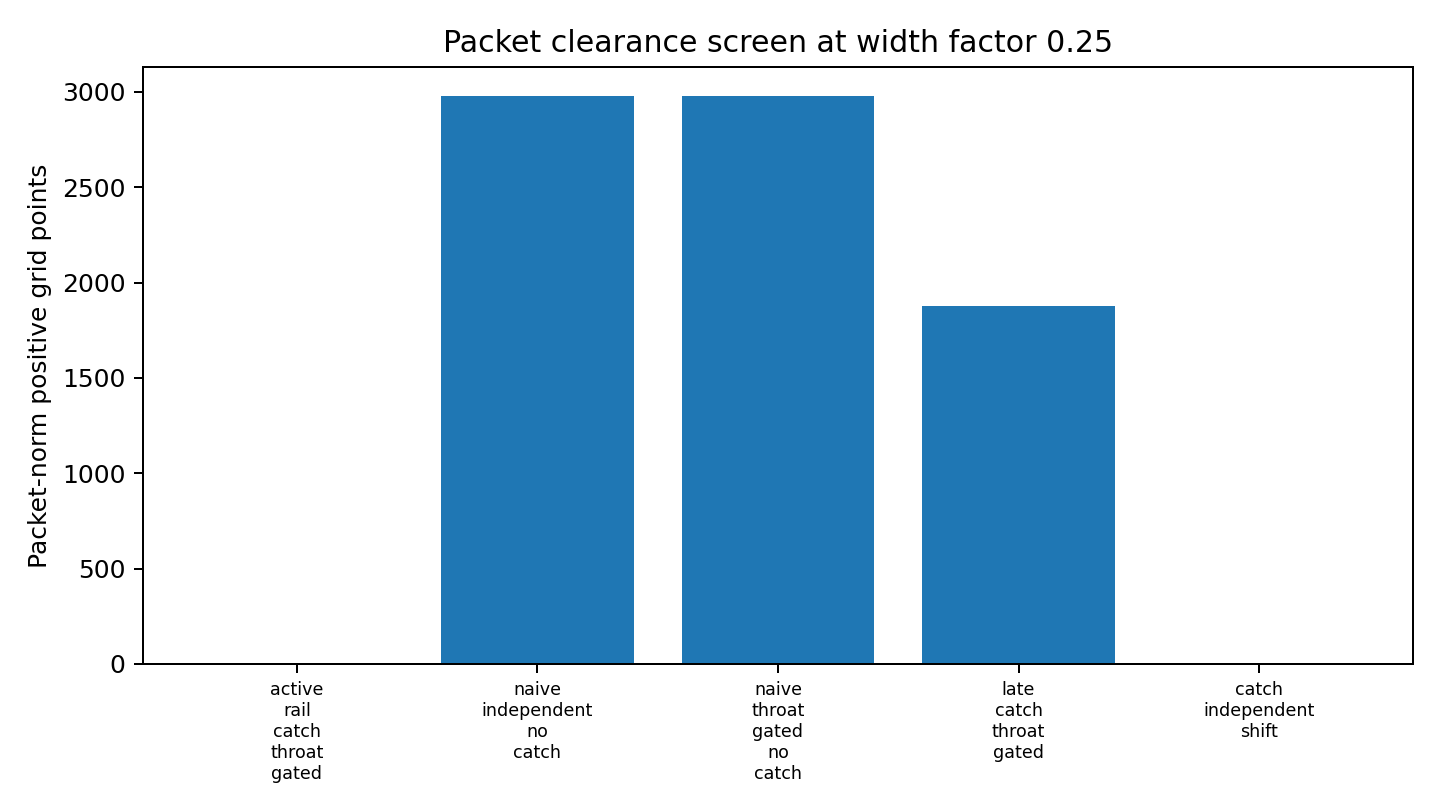
\includegraphics[width=0.78\linewidth]{../figures/packet_positive_points_width025.png}
\caption{Packet-clearance diagnostic for the width-$0.25$ screen. Catch-rematched branches preserve zero packet-norm-positive grid points; unrematched and late-catch branches enter packet-norm-positive regions.}
\label{fig:packetpositive}
\end{figure}

\begin{figure}[H]
\centering
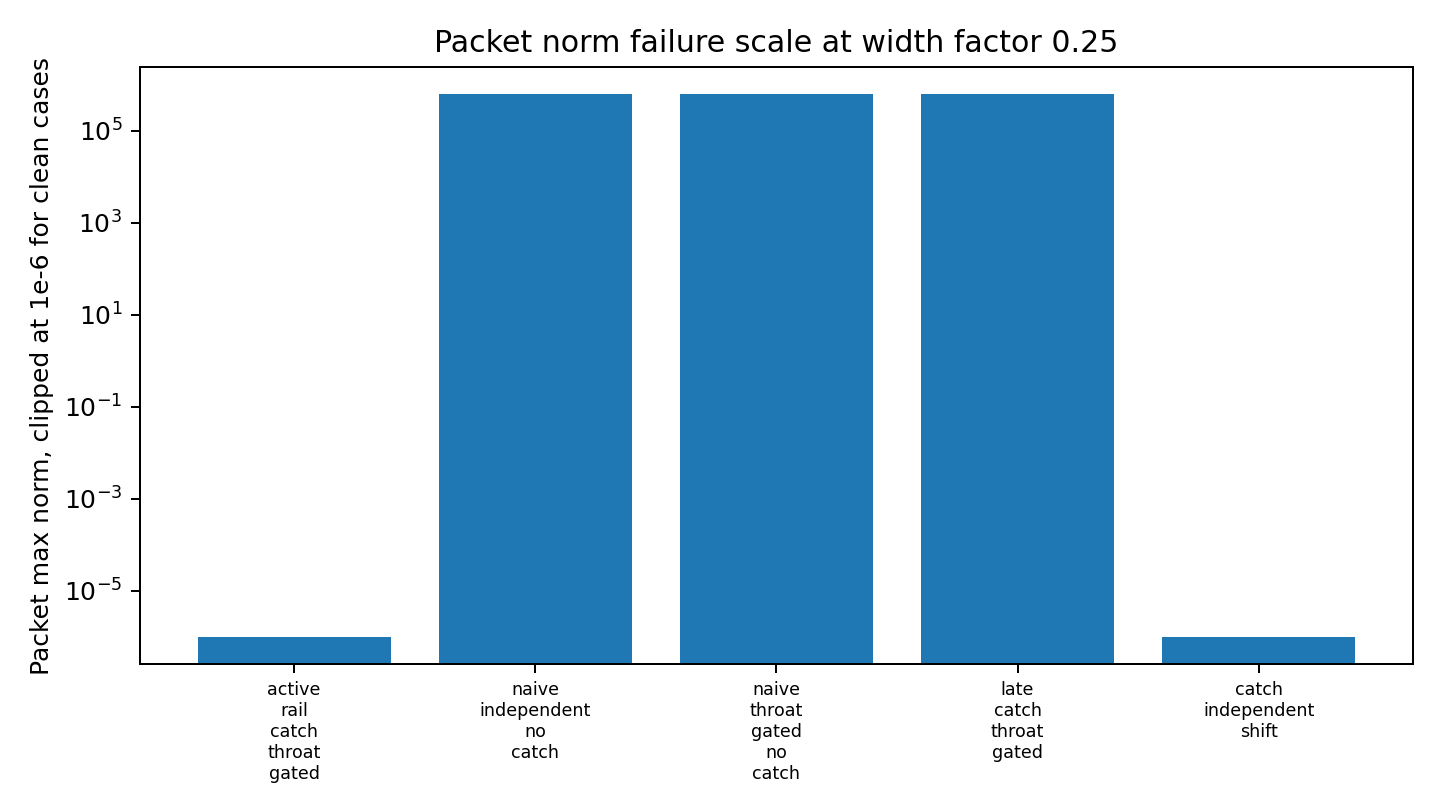
\includegraphics[width=0.78\linewidth]{../figures/packet_max_norm_width025.png}
\caption{Packet norm scale for the width-$0.25$ screen. Clear branches are clipped at $10^{-6}$ for log-scale visibility; failed branches reach large positive norms.}
\label{fig:packetmax}
\end{figure}



\section{What the screen establishes}

The strongest result in the reduced diagnostic is the service-order result. The packet remains timelike when it is caught before release. In unrematched service the packet stays fast while the release layer changes beneath it. In late-catch service the plant withdraws the support sequence before the packet has been rematched. The packet norm enters large positive regions in both cases.

The catch-rematched independent-shift branch also remains packet-clear in this specific screen. That result is useful because it tells us what the screen is isolating. It isolates packet-service timing. The shift-containment rule comes from the gated-shift sweep, where independent passenger shift and throat-gated shift were compared across traversal and exit configurations. The present screen adds the service rule: after shift allocation has been set, catch/rematch is the packet-critical event.

The packet-clearance figures make the service distinction visible. Packet-positive points vanish in catch-rematched service and appear in the unrematched and late-catch branches. Packet max norm stays negative in cleared branches and rises by orders of magnitude in failed branches. The radial null-speed and bundle-compression diagnostics play a different role. They remain in the data products as first reduced clearance checks for immediate radial pileup or folding in the tested service window.

Together, the gated-shift result and the packet-service screen give the rail two constructive rules. Transport shift belongs inside the support envelope. The packet is caught before release. Those rules turn the interface into a division of labor: the plant holds transport structure, the packet receives timed service, the rail condition keeps shift inside support, and the throat relaxes after the packet-critical stage has passed.

\section{Engineering meaning under source availability}

The source-availability assumption is the frame that makes the engineering question sharp. Standard wormhole and warp-drive literature gives a discouraging first impression because the source problem dominates the view: exotic support, quantum-inequality pressure, wall severity, horizon structure, chronology, and semiclassical backreaction all crowd the foreground. Under that view, the practical engineering picture can look like one undifferentiated impossibility: too much negative energy, too thin a wall, too much causal trouble, too little control.

The supplied-source question is conditional and concrete. If the needed support is available as infrastructure, does the remaining transit architecture organize into a coherent, tunable service? The reduced results increase confidence in that conditional possibility. The hard transport problem separates into jobs. Shift containment keeps transport inside the support envelope. Catch/rematch protects the packet before release. Radial and angular capacity move different burden channels. The support edge becomes a managed region. The packet worldtube becomes the passenger object.

That separation matters because engineering feasibility begins when a global difficulty becomes a set of local controls. Under the supplied-source premise, the geometry becomes a system with identifiable actuators, failure modes, margins, and regions of responsibility. The active-rail branch gives the constructive object: the throat carries the rail, the packet is caught, the release is timed, and the dangerous gradients are assigned to infrastructure.

This is the confidence shift. The literature makes the source gate severe, and that severity remains decisive. The active-rail result shows that the supplied-source branch has internal structure. It gives future source work a layout: core throat support, shift-release layer, catch layer, angular capacity sector, support edge, shoulder, reset. A source model can be asked to supply specific jobs in specific regions instead of a single undifferentiated exotic demand.

\section{Next gates and new questions}

The next gates carry the same structure forward. A constraint-quality construction tests whether the rail can be supplied without singular or unbounded stress layers. The reduced metric has to be embedded in, or replaced by, a $3+1$ construction satisfying the Hamiltonian and momentum constraints with admissible source behavior. That calculation requires more computational reach than the radial diagnostic model and becomes the natural next stage because it tests the service geometry as a spacetime construction.

A global causal calculation tests whether the catch and release choreography stays clear beyond the radial screen. Off-axis null congruences, packet-boundary geodesic families, and searches for horizon or Cauchy-horizon behavior should focus on the catch, shift-fade, support-edge, and relaxation layers. This is the direct continuation of the Garattini--Zatrimaylov comparison: the localized-bubble obstruction lives where shell and throat interact, so the active rail must be tested where packet boundary, shift envelope, and throat support edge meet.

A semiclassical stress calculation tests the quantum response of the rail. Finazzi, Liberati, and Barcelo show that dynamically formed superluminal warp drives can develop semiclassical instability pressure \citep{finazzi_liberati_barcelo_2009}. The active rail changes the object under study and gives that test a clearer target: the support-contained shift edge, the catch layer, the packet exposure, and the reset shoulder.

Repeated-operation studies then ask whether the plant resets cleanly. They ask how wide the service interval has to be, how smooth the support edge must remain, how much angular capacity relieves spatial curvature near the packet, which source channel carries transition current, and whether hidden ledgers accumulate in the shoulder or edge. These questions carry the architecture forward because they inherit the same physical geography: packet, rail, edge, release, reset.

\section{Conclusion}

A wormhole and a warp drive usually enter the imagination from opposite directions. The wormhole feels like architecture: a throat, a bridge, a passage held open by strange and costly support. The warp drive feels like motion: a ship, a bubble, a moving distortion that carries its passengers by reshaping the space around them. The original interface question asked whether those pictures could meet in one physical idea: whether the supported throat and the transport shift could belong to the same transit system.

Garattini and Zatrimaylov give that question a sharper boundary. Their wormhole--warp-drive correspondence places the interface on formal ground and identifies the obstruction faced by localized Alcubierre bubbles in Morris--Thorne wormhole backgrounds. Their result now provides the sharpest comparison point for the architecture developed here. The active-rail construction belongs to the structured-background side of the correspondence, where intrinsic curvature, support geometry, and transport shift are treated as parts of one system.

The present work develops that constructive branch as a throat-supported shift rail. The throat prepares the support envelope, carries the shift, supplies capacity and lapse margin, receives the packet, catches it, releases the transport field, and relaxes afterward. The passenger occupies a finite packet worldtube inside that service. The geometry becomes more than a passage and more than a moving transport shell. It becomes a plant with a sequence: prepare, carry, catch, release, relax, reset.

The source-availability assumption is the frame that makes the engineering question sharp. Standard wormhole and warp-drive literature gives a discouraging first impression because the source problem dominates the view: exotic support, quantum-inequality pressure, wall severity, horizon structure, chronology, and semiclassical backreaction all crowd the foreground. Under that view, the practical engineering picture can look like one undifferentiated impossibility: too much negative energy, too thin a wall, too much causal trouble, too little control. The conditional engineering question studied here asks what remains when the needed support is treated as supplied infrastructure: does transit organize into a coherent, tunable service architecture?

The reduced results increase confidence in that conditional engineering possibility. They show that the hard transport problem separates into jobs. Shift containment keeps transport inside the support envelope. Catch/rematch protects the packet before release. Radial and angular capacity move different burden channels. The support edge becomes a managed region. The packet worldtube becomes the passenger object. That separation matters because engineering feasibility begins when a global difficulty becomes a set of local controls.

Under the supplied-source premise, the architecture changes the meaning of feasibility. Source supply remains the decisive physics gate, and the present work gives the supplied-source branch a concrete service form. Once support is admitted as an input, the geometry becomes a system with identifiable actuators, failure modes, margins, and regions of responsibility. The standard literature makes the combined wormhole/warp picture look naturally severe when it is imagined as a localized bubble crossing a throat or as an unsupported wall moving with the passenger. The active-rail branch gives the constructive alternative: the throat carries the rail, the packet is caught, the release is timed, and the dangerous gradients are assigned to infrastructure.

The reduced diagnostic screen gives this picture its first technical bite. In the stressed service cases, caught branches preserve packet clearance while no-catch and late-catch comparison branches lose it. The result identifies the first packet-service rule: the packet is caught before the rail releases it. The earlier gated-shift sweep supplies the companion rule: transport shift belongs inside its support envelope. Together, these rules give the architecture its spine. Transport is supported by the throat, and release is timed around the packet.

This is the design's most interesting feature. It changes the engineering object. The throat becomes a machine that performs a service. The packet worldtube, support edge, shift-release layer, catch layer, angular capacity sector, and reset shoulder become regions with physical jobs. The architecture gives future calculations specific places to look and specific failures to test.

The next gates carry that same structure forward. A constraint-quality construction tests whether the rail can be supplied without singular or unbounded stress layers. A global null-congruence calculation tests whether the catch and release choreography stays clear away from the radial screen. A semiclassical stress calculation tests whether the shift/support edge remains calm under quantum backreaction. Repeated-operation studies ask whether the plant resets cleanly or accumulates hidden ledgers in the shoulder and edge. These are heavier calculations, and they require more computational reach than the reduced radial screen. They are also natural continuations of the same machine: packet, rail, edge, release, reset.

The path from the 2022 inquiry to the present architecture is therefore a real progression. The early question pointed at the interface. Garattini and Zatrimaylov gave the interface a formal boundary. The active-rail construction develops the structured branch into a service geometry. Under source availability, the work raises confidence that some engineering-feasible transit architecture may exist because the burden can be organized instead of merely endured. The result is a packet-centered transit architecture in which warp-like shift becomes a supported throat operation and traversal becomes a timed rail service through active infrastructure.

\begin{thebibliography}{99}

\bibitem[Goldman(2022)]{goldman_2022_inquiry}
Daniel S. Goldman.
\newblock \emph{An Inquiry on Warp Drives and Wormholes}.
\newblock ResearchGate/OSF preprint, 2022. doi:10.31219/osf.io/sre5z.

\bibitem[Morris and Thorne(1988)]{morris_thorne_1988}
Michael S. Morris and Kip S. Thorne.
\newblock Wormholes in spacetime and their use for interstellar travel: A tool for teaching general relativity.
\newblock \emph{American Journal of Physics}, 56:395--412, 1988. doi:10.1119/1.15620.

\bibitem[Morris et~al.(1988)]{morris_thorne_yurtsever_1988}
Michael S. Morris, Kip S. Thorne, and Ulvi Yurtsever.
\newblock Wormholes, time machines, and the weak energy condition.
\newblock \emph{Physical Review Letters}, 61:1446--1449, 1988. doi:10.1103/PhysRevLett.61.1446.

\bibitem[Ford and Roman(1996)]{ford_roman_1996}
L. H. Ford and Thomas A. Roman.
\newblock Quantum field theory constrains traversable wormhole geometries.
\newblock \emph{Physical Review D}, 53:5496--5507, 1996. doi:10.1103/PhysRevD.53.5496.

\bibitem[Fewster and Roman(2005)]{fewster_roman_2005}
Christopher J. Fewster and Thomas A. Roman.
\newblock On wormholes with arbitrarily small quantities of exotic matter.
\newblock \emph{Physical Review D}, 72:044023, 2005. doi:10.1103/PhysRevD.72.044023.

\bibitem[Hochberg and Visser(1998)]{hochberg_visser_1998}
David Hochberg and Matt Visser.
\newblock The null energy condition in dynamic wormholes.
\newblock \emph{Physical Review Letters}, 81:746--749, 1998. doi:10.1103/PhysRevLett.81.746.

\bibitem[Alcubierre(1994)]{alcubierre_1994}
Miguel Alcubierre.
\newblock The warp drive: hyper-fast travel within general relativity.
\newblock \emph{Classical and Quantum Gravity}, 11:L73--L77, 1994. doi:10.1088/0264-9381/11/5/001.

\bibitem[Pfenning and Ford(1997)]{pfenning_ford_1997}
Michael J. Pfenning and L. H. Ford.
\newblock The unphysical nature of warp drive.
\newblock \emph{Classical and Quantum Gravity}, 14:1743--1751, 1997. doi:10.1088/0264-9381/14/7/011.

\bibitem[Natario(2002)]{natario_2002}
Jose Natario.
\newblock Warp drive with zero expansion.
\newblock \emph{Classical and Quantum Gravity}, 19:1157--1165, 2002. doi:10.1088/0264-9381/19/6/308.

\bibitem[Van Den Broeck(1999)]{van_den_broeck_1999}
Chris Van Den Broeck.
\newblock A warp drive with more reasonable total energy requirements.
\newblock \emph{Classical and Quantum Gravity}, 16:3973--3979, 1999. doi:10.1088/0264-9381/16/12/314.

\bibitem[Everett and Roman(1997)]{everett_roman_1997}
Allen E. Everett and Thomas A. Roman.
\newblock Superluminal subway: The Krasnikov tube.
\newblock \emph{Physical Review D}, 56:2100--2108, 1997. doi:10.1103/PhysRevD.56.2100.

\bibitem[Bobrick and Martire(2021)]{bobrick_martire_2021}
Alexey Bobrick and Gianni Martire.
\newblock Introducing physical warp drives.
\newblock \emph{Classical and Quantum Gravity}, 38:105009, 2021. doi:10.1088/1361-6382/abdf6e.

\bibitem[Fuchs et~al.(2024)]{fuchs_2024}
Jared Fuchs, Christopher Helmerich, Alexey Bobrick, Luke Sellers, Brandon Melcher, and Gianni Martire.
\newblock Constant velocity physical warp drive solution.
\newblock \emph{Classical and Quantum Gravity}, 41:095013, 2024. doi:10.1088/1361-6382/ad26aa.

\bibitem[Finazzi et~al.(2009)]{finazzi_liberati_barcelo_2009}
Stefano Finazzi, Stefano Liberati, and Carlos Barcelo.
\newblock Semiclassical instability of dynamical warp drives.
\newblock \emph{Physical Review D}, 79:124017, 2009. doi:10.1103/PhysRevD.79.124017.

\bibitem[Gao et~al.(2017)]{gao_jafferis_wall_2017}
Ping Gao, Daniel Louis Jafferis, and Aron C. Wall.
\newblock Traversable wormholes via a double trace deformation.
\newblock \emph{Journal of High Energy Physics}, 2017:151, 2017. doi:10.1007/JHEP12(2017)151.

\bibitem[Garattini and Zatrimaylov(2024)]{garattini_zatrimaylov_2024}
Remo Garattini and Kirill Zatrimaylov.
\newblock On the wormhole-warp drive correspondence.
\newblock \emph{Journal of Cosmology and Astroparticle Physics}, 2024(08):061, 2024. doi:10.1088/1475-7516/2024/08/061.

\bibitem[Chowdhury(2025)]{chowdhury_2025}
Abhishek Chowdhury.
\newblock Warp drives and Martel--Poisson charts.
\newblock \emph{European Physical Journal C}, 85:112, 2025. doi:10.1140/epjc/s10052-025-13831-9.

\end{thebibliography}
\end{document}
